\documentclass[../main/main.tex]{subfiles}
\begin{document}

\section{Maps of \rss\ and \hnn}

In the following we will assume the \rss\ that we will consider to be \cpt\ and connected. Let $f\colon X\to Y$ be a non-\const\ \holo\ map of \rss\ (hence surjective\footnote{\cite[Thm. 4.3.1]{CM}})

\begin{definition}
	\begin{itemize}
		\item The \emph{ramification index} of $f$ at $x\in X$ is the integer $k_x\in\Z_{\geq1}$ \st $f$ is locally of the form $z^k$, where $z$ is a local coordinate centered in $x$. 
		\item The \emph{differential length} of $f$ at $x\in X$ is $\nu_x=k_x-1$.
		\item A point $x\in X$ \st $\nu_x>0$ is called a \emph{ramification point}. The \emph{ramification locus} of $f$ is the set of its ramification points. If $\n_x=0$ we say that $f$ is \emph{unramified} at $x$. If $\n_x=1$ we say that $f$ has \emph{simple ramification} at $x$. 
		\item If $x\in X$ is a ramification point, then $f(x)\in Y$ is called a \emph{branch point}. The \emph{branch locus} $B_f$ of $f$ is the set of its branch points.
	\end{itemize}
\end{definition}

The ramification locus and branch locus are finite sets of $X$ and $Y$ respectively.\footnote{\cite[Lemma 4.2.5.]{CM}} We assume $f$ non-\const. For any $y,y'\in Y\setminus B_f$ we have $|\inv f(y)|=|\inv f(y')|$.\footnote{\cite[Thm. 4.3.3]{CM}} We call \emph{degree} of $f$ the integer $\deg f\defeq|\inv f(y)|$ for any $y\in Y\setminus B_f$. Then:

\begin{theorem}[Riemann-Hurwitz {\cite[Thm. 4.4.1]{CM}}]
	Let $g_X$ and $g_Y$ denote the genus of $X$ and $Y$ respectively. Then
	\deq{\underbrace{2g_X-2}_{\c(X)}=(\underbrace{2g_Y-2}_{\c(Y)})\deg f+\sum_{x\in X}\nu_x}
\end{theorem}

We also have that for any $y\in Y$
\deq{\deg f=\sum_ik_{x_i}}
where $i$ labels the elements of $\inv f(y)=\{x_1,\ldots,x_n\}$. Denote $d\defeq\deg f$. 

\begin{definition}
	Let $y\in Y$, $\inv f=\{x_1,\ldots,x_n\}$. We call \emph{ramification profile} of $f$ at $y$ the partition of $d$ given by $(k_{x_1},\ldots,k_{x_n})$. We say that $f$ is \emph{unramified} / \emph{simply ramified} / \emph{fully ramified} if its ramification profile is $(1,\ldots,1)$ / $(2,1,\ldots,1)$ / $(d)$ respectively.
\end{definition}

\begin{definition}
	Two \holo\ maps of \rss\ $f\colon X\to Y$ and $g\colon\ti X\to Y$ are called \emph{isomorphic} if there is an {isomorphism} of \rss\ $\f\colon X\to\ti X$ \st $f=g\circ \f$. 
	
	An \emph{automorphism} of $f\colon X\to Y$ is an automorphism $\p\colon X\to X$ \st $f=f\circ \p$. The group of automorphisms of $f$ is denoted $\Aut(f)$. 

\end{definition}

\begin{definition}
	Let $Y$ be a connected \cpt\ \rs\ of genus $g$, $B=\{b_1,\ldots,b_n\}\subset Y$ finite subset, $d\in\Z_{\geq1}$, $\q_1,\ldots,\q_n\prt d$. We define the \emph{(degree $d$) connected Hurwitz number} to be 
	\deq{H^\circ_{h\overset d\to g}(\q_1,\ldots,\q_n):=\sum_{[f]}\frac1{|\Aut(f)|}}
	and the \emph{(degree $d$) Hurwitz number} to be
	\deq[eq:disc-H-numb]{H^\bullet_{h\overset d\to g}(\q_1,\ldots,\q_n):=\sum_{[f]}\frac1{|\Aut(f)|}}
	where both sums runs over isomorphism classes of \holo\ maps $f\colon X\to Y$ \st
	\begin{itemize}
		\item $X$ is a \cpt\ \rs\ of genus $h$\footnote{For $X$ disconnected, its genus is defined by $\c=2g-2$, where the Euler characteristic $\c$ is naturally additive under disjoint unions. The Riemann-Hurwitz formula then applies identically in also for $X$ disconnected.}
		\item the branch locus of $f$ is $B$
		\item the ramification profile of $f$ at $b_i$ is $\q_i$
	\end{itemize}
	In the case of connected Hurwitz numbers we further require $X$ to be connected. Numbers \eqref{eq:disc-H-numb} are also called \emph{disconnected Hurwitz number} since $X$ is allowed to be disconnected.
\end{definition}

Note that for any $f\colon X\to Y$ as in the definition above we have 
\deq{\sum_{x\in X}\n_x=\sum_{i=1}^n(d-\ell(\q_i))=nd-\sum_{i=1}^n\ell(\q_i)}
where $\ell(\q_i)$ denotes the length of the partition $\q_i$ (\ie the number of cycles in $\q_i$), so due to Riemann-Hurwitz theorem we have 
\deq[eq:RHgenus]{2h-2=(2g-2)d+nd-\sum_{i=1}^n\ell(\q_i)}
In particular the ramification profile of $f:X\to Y$ and the genus of $Y$ uniquely determines the genus of $X$. 

\section{Maps of \rss\ as ramified covers}

Maps of \rss\ are ramified covers:

\begin{definition}
	A \emph{ramified cover} is a continuous function between compact topological surfaces $f\colon X\to Y$ with a finite set $B\subset Y$ \st
	\begin{itemize}
		\item$\inv f(B)$ is finite,
		\item $f\colon X\setminus\inv f(B)\to Y\setminus B$ is a covering.
	\end{itemize}
\end{definition}

Vice-versa, we have

\begin{theorem}[Riemann's Existence Thm. {\cite[Thm. 6.2.2]{CM}}] 
	Let $Y$ \cpt\ \rs, $X^0$ topological surface, $\{b_1,\ldots,b_n\}\subset Y$ finite subset, $f^0\colon X^0\to Y\setminus\{b_1,\ldots,b_n\}$ covering of finite degree. Then there exists a unique (up to isomorphisms) \cpt\ \rs\ $X$ \st
	\begin{itemize}
		\item $X^0$ is a dense subset of $X$,
		\item $f^0$ extends to a \holo\ map of \rss\ $f\colon X\to Y$.
	\end{itemize}
\end{theorem}

\begin{definition}
	The map $f\colon X\to Y$ is said \emph{$y_0$-labelled} if $y_0\in Y\setminus B_f$ and is chosen an isomorphism $L\colon \inv f(y_0)\to \{1,\ldots,d\}$. We also say that $L$ is a \emph{labelling}. An \emph{isomorphism of $y_0$-labelled maps} $(f,L)$ and $(f',L')$ is an isomorphism of \rss\ $\f\colon X\to X'$ \st 
	\deq{f'\circ\f=f\tand L'\circ\f=L}
\end{definition}

\begin{definition}
	A $y_0$-labelled map $f\colon X\to Y$ determines a group homomorphism 
	\deq{
		\F\colon\u_1(Y\setminus B_f,y_0)\to S_d\tcomma \g\mapsto\s_\g
	}
	called \emph{monodromy representation}.
\end{definition}

We have that $(f,L)\cong(f',L')$ imply $\F=\F'$.


Now consider $b\in B_f$ and $\g\in\u_1(Y\setminus B_f,y_0)$ simple loop winding once around $b$ (and with zero winding number around the other branch points). If the ramification profile of $f$ at $b$ is $\q=(k_1,\ldots,k_l)$, then $\s_\g$ has cycle type $\q$ (to see this recall that the local expression of $f$ around ramification points is $z^k$ and consider a circle around $y_0$ of unit radius in the chart).

\begin{definition}
	Let $Y$ be a connected \rs\ of genus $g$, $y_0,b_1,\ldots,b_n\in Y$ points, $d\in\Z_{\geq1}$ and $\q_1,\ldots,\q_n\prt d$. A \emph{monodromy representation of type} $(g,d,\q_1,\ldots,\q_n)$ is a group homomorphism $\F\colon\u_1(Y\setminus\{b_1,\ldots,b_n\},y_0)\to S_d$ \st if $\g_k$ is a small loop around $b_k$ then $\F(\g_k)$ has cycle type $\q_k$.
	
	If moreover the subgroup $\im \F\subset S_d$ acts transitively on $\{1,2,\ldots,d\}$ we say that $\F$ is a \emph{connected monodromy representation of type} $(g,d,\q_1,\ldots,\q_n)$.
	
\end{definition}

Note that if two labellings $L,L'$ of $f\colon X\to Y$ are given, then $L'=\s\cdot L$ for some $\s\in S_d$ and $\F'(\g)=\s\cdot\F(\g)\cdot\inv\s$. In particular the type of the monodromy representation does note depend on the chosen labelling. 


We obtained that a degree $d$ map $f\colon X\to Y$ between \cpt\ connected \rss\ \st the ramification profile over each branch point is $\q_i$ gives rise to a connected monodromy representation $\F$ of type $(g_Y,d,\q_1,\ldots,\q_n)$. If we let $X$ to be non connected, then the monodromy representation may not be connected anymore, more precisely: the monodromy representation is connected \tiff $X$ is connected.\footnote{For further details: \cite[§§7.1]{CM}.} We also have that isomorphic maps give the same monodromy representation. 

Conversely:

\begin{theorem}[{\cite[Thm. 7.2.2]{CM}}]
	Let $Y$ be a \rs\ of genus $g$, $\F$ a monodromy representation of type $(g,d,\q_1,\ldots,\q_n)$, $B=\{b_1,\ldots,b_n\}\subset Y$ a finite subset. Then exists a $y_0$-labelled \holo\ map of \rs\ covering $Y$ with branch locus $B$ whose associated monodromy is $F$. Such map is unique up to isomorphisms of $y_0$-labelled maps. 
\end{theorem}
\begin{proof}[Sketch of proof]
	In the proof of this result the Riemann's Existence theorem is fundamental. We construct explicitly the topological space $X_0$ and the covering $f^0\colon X^0\to Y\setminus B$ in such a way that the map $f\colon X\to Y$ given by the Riemann's Existence theorem has the desired monodomy representation. 
	
	Take cycles $\a_1,\ldots\a_g,\b_1,\ldots,\b_g$ in $Y$ generating $\pi_1(Y,y_0)$ all containing a point $p\in Y$ in such a way that $Y\setminus\{\a_1,\ldots\a_g,\b_1,\ldots,\b_g\}$ is the fundamental polygon describing $Y$. Denote by $\g_i$ a loop containing $y_0$, winding once around $b_i$, never around the other elements of $B$, and fully contained in $Y\setminus\{\a_1,\ldots\a_g,\b_1,\ldots,\b_g\}$.
	
	

	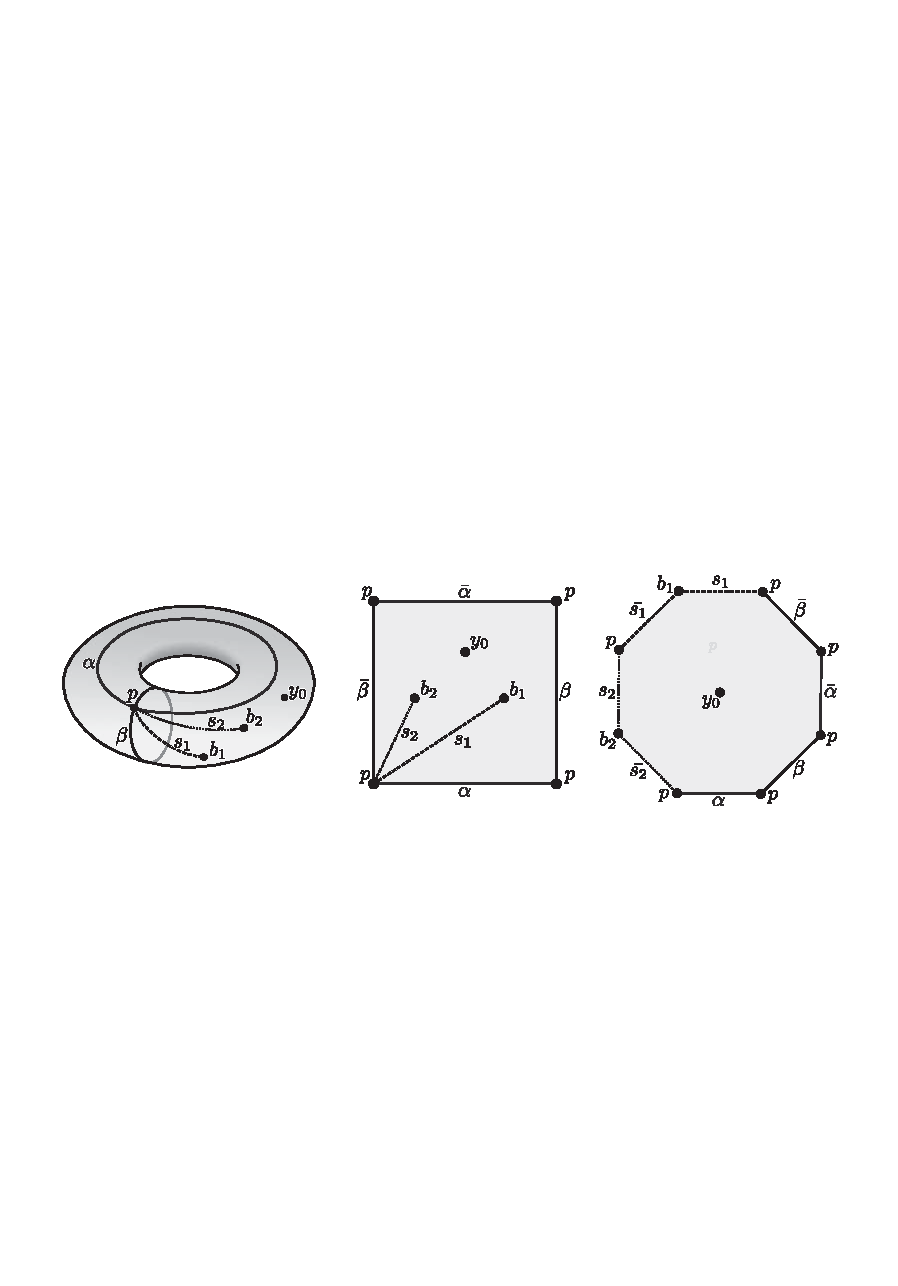
\includegraphics[]{../figures/CM-fig-7-6.pdf}
	
	Consider segments $s_j$ connecting $p$ with the points $b_j$. Open the previous polygon in correspondence of these segments, so that we get a new polygon
	\deq{P:=s_1\ba{s}_1\cdots s_n\ba{s}_n\a_1\b_1\ba{\a}_1\ba{\b}_1\cdots\a_g\b_g\ba{\a}_g\ba{\b}_g}
	Then it suffices to take $d$ copies of $P$ and glue their boundaries appropriately to produce $X^0$ in such a way that the natural projection to $Y\setminus B$ has the desired monodromy representation:
	\deq{s_{j,k}&\sim\ba s_{j,\F(\g_j)(k)}\\
		\ba\a_{i,k}&\sim \a_{i,\F(\b_i)(k)}\\
		\b_{i,k}&\sim \ba\b_{i,\F(\a_i)(k)}}
\end{proof}

The previous theorem ensures that we have a bijection between isomorphism classes of $y_0$-labeled Hurwitz covers and connected monodromy representations of type $(g,d,\q_1,\ldots,\q_n)$. Then we can prove

\begin{theorem}[{\cite[Thm. 7.3.1, Thm. 7.3.2]{CM}}]\label{thm:CM7.3.1}
	Let $M^\circ$ (resp $M^\bullet$) be the set of connected monodromy representations (resp. monodromy representations) of type $(g,d,\q_1,\ldots,\q_n)$. Then
	\deq{H^\circ_{h\overset d\to g}(\q_1,\ldots,\q_n)=\frac{|M^\circ|}{d!}}
	and
	\deq{H^\bullet_{h\overset d\to g}(\q_1,\ldots,\q_n)=\frac{|M^\bullet|}{d!}}
	where $h$ is determined by \eqref{eq:RHgenus}. 
\end{theorem}

\begin{proof}[Sketch of proof]
	We give the proof in the connected case, the other case is analogous. 
	
	Take $f\colon X\to Y$ Hurwitz cover. Clearly there are $d!$ possible choices of a $y_0$-labelling $L\colon \inv f(y_0)\to \{1,\ldots,d\}$. An automorphism $\f\in\Aut(f)$ is an isomorphism $\f\colon X\overset\sim\to X$ satisfying $f=f\circ\f$. In particular $\f$ gives an isomorphism $(f,L)\cong(f,L')$ where $L'=\f\cdot L:=L\circ\inv\f$. Here $\f\cdot L$ denotes the left action of $\Aut(f)$ on the possible $y_0$-labellings of $f$. Such action is free (\ie $\f\cdot L=L$ imply $\f=\id_X$) so the number of isomorphism classes of $y_0$-labelings of $f$ is $d!/|\Aut(f)|$. 
	
	From the previous theorem isomorphism classes of $y_0$-labelled maps for the given $f$ are in bijection with the distinct monodromy representations arising from $f$ by different labelings of $\inv f(y_0)$. Therefore 
	\deq{m_f=\frac{d!}{|\Aut(f)|}}
	where $m_f$ the number of distinct monodromy representations arising from $f$ by different labelings of $\inv f(y_0)$. So we have
	\deq{H^\circ_{h\overset d\to g}(\q_1,\ldots,\q_n):=\sum_{[f]}\frac1{|\Aut(f)|}=\sum_{[f]}\frac{m_f}{d!}=\frac{|M^\circ|}{d!}}
\end{proof}

Although the information carried by connected Hurwitz numbers is usually more interesting for geometrical purposes, it turns out that it is easier to compute the (possibly disconnected) Hurwitz numbers. We will see later how it is possible to recover the connected Hurwitz numbers from the disconnected ones. 

We mention that using some ``degeneration formulas'' (which heuristically correspond to shrink the \rs\ Y producing nodal curves) all disconnected degree $d$ Hurwitz numbers are determined in therms of Hurwitz numbers of the form $H^\bullet_{h\overset d\to0}(\q_1,\q_2,\q_3)$.\footnote{\cite[Thm. 7.5.3]{CM}} For this reason (and others) we later restrict our discussion to the case $g=0$. 

\section{Interlude: representation theory of $S_d$}

Using theorem \ref{thm:CM7.3.1} the problem of computing degree $d$ Hurwitz numbers can be translated into a problem in representation theory of the symmetric group $S_d$. In order to show this we need some facts about representation theory (see \cite[Part I]{FH}, \cite{M} and \cite[§8]{CM} for more details). 

\begin{definition}
	The \emph{group algebra} of the symmetric group $S_d$ is the complex algebra generated by the elements of $S_d$, that is
	\deq{\C[S_d]:=\left\{\sum_{\s\in S_d}a_\s\s\ \big|\  a_\s\in\C\right\}}
	with operations
	\deq{\sum_{\s\in S_d}a_\s\s+\sum_{\s\in S_d}b_\s\s=\sum_{\s\in S_d}(a_\s+b_\s)\s}
	\deq[eq:formal-expansion]{\bigg(\sum_{\s\in S_d}a_\s\s\bigg)\cdot\bigg(\sum_{\s\in S_d}b_\s\s\bigg)=\sum_{\s\in S_d}\sum_{\s'\in S_d}a_\s b_{\s'}(\s\cdot\s')}
	\deq{t\cdot\bigg(\sum_{\s\in S_d}a_\s\s\bigg)=\sum_{\s\in S_d}(t a_\s)\s}
	where $t\in\C$. Expression in the \rhs of \eqref{eq:formal-expansion} (before multiplying $\s$ and $\s'$) is called formal expansion of the product.
	
	We define \emph{class algebra} of $S_d$ the center of the group algebra
	\deq{	\cZ\C[S_d]&=\{x\in\C[S_d]\ \big|\ yx=xy\tforall y\in\C[S_d]\}}
\end{definition}

The following functions are very important for our discussion:

\begin{definition}
	A \emph{class function} on $S_d$ is a map $\a\colon S_d\to\C$ which is constant on conjugacy classes, i.e. $\forall h\in S_d$ we have $\a(\inv hgh)=\a(h)$. Let $\C_\tclass$ denote the vector space of class functions on $S_d$. We define on $\C_\tclass$ the following Hermitian inner product
	\deq[eq:inner-prod-cfunc]{(\a,\b):=\frac1{d!}\sum_{\s\in S_d}\a(\s)\overline{\b(\s)}=\frac1{d!}\sum_{C\subset S_d}|C|\a(C)\overline{\b(C)}}
 	for any $\a,\b\in \C_\tclass$, where $\sum_C$ runs over the conjugacy classes of $S_d$. 
\end{definition}

We have the following

\begin{lemma}[{\cite[§§3.4]{FH}}]
	\deq{\cZ\C[S_d]=\left\{\sum_{\s\in S_d}\a(\s)\s\ \big|\  \a\in\C_\tclass\right\}}
\end{lemma}

For $\q\prt d$ denote by $C_\q\subset S_d$ the conjugacy class corresponding to all elements of cycle type $\q$.  Let $\a_\q\colon S_d\to\C$ the class function which takes value 1 on elements of $C_\q$ and 0 otherwise. It is clear that the set $\{\a_\q\ |\ \q\prt d\}$ gives a basis of $\cclass$. Let $c_\q\in\cZ\C[S_d]$ denote the corresponding element in the center of the group algebra, that is 
\deq{c_\q=\sum_{s\in S_d}\a_\q(\s)\s=\sum_{\s\in C_\q}\s}
We get that $\{c_\q\ |\ \q\prt d\}$ form a basis of $\cZ\C[S_d]$ as a complex vector space, called \emph{conjugacy class basis}
\deq{\cZ\C[S_d]=\bigoplus_{\q\prt d}\la c_\q\ra_\C}
Note that the identity element $c_e$ in $\cZ\C[S_d]$ corresponds to the partition $e=(1,\ldots,1)$. 


A (complex) representation of $S_d$ is a homomorphism $\r\colon S_d\to\Aut(V_\r)$ making the finite dimensional complex vector space $V_\r$ into a $S_d$-module. We define the dimension of the representation to be $\dim \r:=\dim_\C V_\r$. Given any representation $\r$, notice that this extends to a homomorphism $\C [S_d]\to\End(V_\r)$, making $V_\r$ into a $\C [S_d]$-module. 

Representations of $S_d$ are described by their characters, which are defined as follows:

\begin{definition}
	Let $\r$ be a representation of $S_d$. The \emph{character} of $\r$ is the class function $\c_\r\in\cclass$ defined by
	\deq{\c_\r(\s):=\tr(\r(\s))}
\end{definition}

The fact that $\c_\r$ is a class function follows from the cyclicity of the trace. From the definition it follows that $\c_\r$ does not depend on the choice of basis for $V_\r$ (due to the corresponding property of the trace) and that $\c_\r(e)=\dim \r$ (since $\r(e)=\id$). It is also easy to see that $\c_{\r_1\oplus\r_2}=\c_{\r_1}+\c_{\r_2}$. 




A representation $\r$ is \emph{irreducible} if $V_\r$ does not contain any nontrivial $S_d$-submodules. For complex representation we have the following fundamental result
\begin{theorem}[{\cite[Thm. 2.12]{FH}}]
	In terms of the inner product \eqref{eq:inner-prod-cfunc} the characters of the irreducible representations of $S_d$ are orthonormal:
	\deq{(\c_{\r_1},\c_{\r_2})=\begin{cases}1\tif \r_1\cong \r_2\\0\tif \r_1\not\cong \r_2\end{cases}}
	where $\r_1,\r_2$ are irreducible representations.  
\end{theorem}

Any complex representation decomposes uniquely into the direct sum of irreducible representations. More precisely, we have
\deq{R=\bigoplus_\r V_\r^{\oplus\dim V_\r}}
where $R$ is the obvious representation of $S_d$ on $\C[S_d]$, called \emph{regular representation}, while the (big) direct sum runs over all the irreducible representations of $S_d$. This also implies the following isomorphism of algebras
\deq{\C[S_d]\cong\bigoplus_\r\End(V_\r)}
which is defined extending $S_d\to\bigoplus_\r\End(V_\r)$ by linearity.

\begin{theorem}[{\cite[Thm. 4.3]{FH}}]
	To each partition $\l\prt d$ corresponds a unique irreducible representation $V_\l$ of $S_d$. The corresponding character, denoted $\c^\l$, is given by Frobenius formula \cite[Eq. 4.10]{FH}. In particular $\c^\l$ is a real class function.
\end{theorem}

By dimensional arguments, we get that characters of irreducible representations form another basis of $\cclass$. Moreover, denoting
\deq{e_\l:=\sum_{\s\in S_d}\c^\l(\s)\s}
we get that $\{e_\l\ |\ \l\prt d\}$ gives another basis of $\cZ\C[S_d]$
\deq{\cZ\C[S_d]=\bigoplus_{\l\prt d}\la e_\l\ra_\C}
which will be called \emph{character basis} or \emph{idempotent basis}. Indeed from characters orthogonality (and the fact that $\overline{\c^\l}=\c^\l$) we get
\deq{e_{\l_i}\cdot e_{\l_j}=\begin{cases}e_{\l_i}\tif e_{\l_i}=e_{\l_j}\\0\quad\text{otherwise}\end{cases}}
Since $\cZ\C[S_d]$ admits a basis of idempotent elements, then it is a \emph{semisimple algebra}. The formulas for the change of basis are given by the characters
\deq[eq:change-basis-class-alg]{e_\l=\frac{\dim \l}{d!}\sum_{\q\prt d}\c^\l(C_\q)c_\q
\quad\tand\quad
c_\q=|C_\q|\sum_{\l\prt  d}\frac{\c^\l(C_\q)}{\dim\l}e_\l}
where $\dim \l:=\dim V_\l$. 

\section{Burnside's formula}

Now we are ready to use the notions that we introduced in order to rewrite the expression of Hurwitz numbers in terms of characters of the irreducible representations of $S_d$. Existence of a idempotent basis for $\cZ\C[S_d]$ and formulas \eqref{eq:change-basis-class-alg} will be crucial. 

Recall that 
\deq{H^\bullet_{h\overset d\to g}(\q_1,\ldots,\q_n)=\frac{|M^\bullet|}{d!}}
where $M^\bullet$ is the set of monodromy representations of type $(g,d,\q_1,\ldots,\q_r)$ with $\q_1,\ldots,\q_n$ partitions of $d$. 

For $\q=\{\q_1,\ldots,\q_{\ell(\q)}\}\prt d$ where $i\in\Z_{\geq1}$ appears $a_i$ times in the partition, $\sum_i ia_i=d$, the size of the centralizer of $C_\q$ is given by
\deq{\fz(\q)=\frac{d!}{|C_\q|}=\prod_{i=1}^{\ell(\q)} a_i! \,i^{a_i}}

In order to account for the case $g\neq0$ one needs 
\begin{definition}
	Let $d\in\Z_{\geq1}$, $\q\prt d$. We define the \emph{kommutator} to be the element
	\deq{\mathfrak K:=\sum_{\q\prt d}\fz(\q)c_\q^2\in\cZ\C[S_d]}
\end{definition}

Then we have the following
\begin{proposition}[{\cite[Prop. 9.2.3]{CM}}]
	\deq{H^\bullet_{h\overset d\to g}(\q_1,\ldots,\q_n)=\frac1{d!}[c_e]\mathfrak K^gc_{\q_n}\cdots c_{\q_2}c_{\q_1}}
	where $[c_e]\mathfrak K^gc_{\q_n}\cdots c_{\q_2}c_{\q_1}$ denotes the coefficient of $c_e$ after writing the product $\mathfrak K^gc_{\q_n}\ldots c_{\q_2}c_{\q_1}$ as a linear combination of the basis elements $c_\q\in\cZ\C[S_d]$. As usual $h$ is determined by Riemann-Hurwitz formula. 
\end{proposition}

By changing basis from the conjugacy basis to the idempotent basis we get

\begin{theorem}[Burnside's Character Formula {\cite[Thm. 9.3.1]{CM}}]
	\deq{H^\bullet_{h\overset d\to g}(\q_1,\ldots,\q_n)=\sum_{\l\prt d}\left(\frac{\dim\l}{d!}\right)^{2-2g}\prod_{i=1}^nf_{C_j}(\l)}
	where
	\deq{f_{C_i}(\l):=|C_i|\frac{\c^\l(C_i)}{\dim \l}}
	and $C_i:=C_{\q_i}$.
\end{theorem}

Recall that from the change of basis formula, 
\deq{c_\q=\sum_{\l\prt d}f_{C_\q}(\l)e_\l}
From Burnside's formula we see that such coefficients $f_{C_\q}(\l)$ for the change of basis correspond to the contribution of the ramification profile $\q$ to the disconnected Hurwitz numbers. 


\section{The generating function}

In the following we will restrict ourselves to the case of $g=0$. Recall that there are some degeneration formulas which allows to express all the Hurwitz numbers in terms of those for $g=0$. For a similar discussion for arbitrary $g$ see \cite[§10]{CM}. We will follow instead \cite[§§2.2,2.3]{O1}. 

For $g=0$ the Riemann-Hurwitz formula implies
\deq[eq:RHgenus0]{2h-2=-2d+nd-\sum_{i=1}^n\ell(\q_i)}
and since this fixes $h$ in terms of $(d,\q_1,\ldots,\q_n)$, we simply denote
\deq{H^\bullet_d(\q_1,\ldots,\q_n):=H^\bullet_{h\overset d\to 0}(\q_1,\ldots,\q_n)=\sum_{\l\prt d}\left(\frac{\dim\l}{d!}\right)^{2}\prod_{i=1}^nf_{C_j}(\l)}
Let $b$ be the number of branch points which have simple ramification, \ie $\q=(2)$. We denote
\deq{H^\bullet_{d,b}(\q_1,\ldots,\q_{n-b}):=H^\bullet_d(\q_1,\ldots,\q_{n-b},\underbrace{(2),\ldots,(2)}_{\text{$b$ times}})=\sum_{\l\prt d}\left(\frac{\dim\l}{d!}\right)^{2}f_2(\l)^b\prod_{i=1}^{n-b}f_{C_j}(\l)}
where $f_2:=f_{C_{(2)}}$. Analogous definitions hold for connected Hurwitz numbers, replacing $H^\bullet$ with $H^\circ$. 

Rather than considering the different Hurwitz numbers separately, it worth to collect them together into generating functions. Fix $m\in\Z_{\geq0}$ to be the number of branch points with non-simple ramification profile. Then

\begin{definition}
	Let $\{p_{i,j}\}$ and $q$ be some variables, $i\in\{1,\ldots,m\}$, $j\in\Z_{\geq0}$. Then we define the \emph{Hurwitz potential} to be\footnote{For $d=0$ we set $H_{d,b}^\bullet(\q_1,\ldots,\q_m)=0$, this is consistent with the fact that there is no covering of degree zero.}
	\deq[eq:Hur-pot-0]{\fH^\bullet(p_{i,j},q,z):=\sum_{d,b=0}^\infty q^d\frac{z^b}{b!}\sum_{\q_1\prt d}\cdots\sum_{\q_{m}\prt d}p_1^{\q_1}\cdots p_{m}^{\q_{m}}H_{d,b}^\bullet(\q_1,\ldots,\q_m)}
	where for $\q=(l_1,\ldots,l_k)\prt d$ we have
	\deq[eq:power-sum-sym-pol]{p^{\q}_i:=(p_{i,1}^{l_1}+\cdots+p_{i,d}^{l_1})\cdots(p_{i,1}^{l_k}+\cdots+p_{i,d}^{l_k})}
	We also introduce the \emph{modified Hurwitz potential} to be
	\deq{\fh^\bullet_d(\q_q,\ldots,\q_m):=\sum_{b=0}^\infty\frac{z^b}{b!}H^\bullet_{d,b}(\q_1,\ldots,\q_m)}
	Analogous definitions hold for the \emph{(modified) connected Hurwitz potential} $\fH^\circ$ and $\fh^\circ$. 
\end{definition}

Note that from the definition we have
\deq{\fH^\bullet(\p_{i,j},q,z)=\sum_{d=0}^\infty q^d\sum_{\q_1\prt d}\cdots\sum_{\q_{m}\prt d}p_1^{\q_1}\cdots p_{m}^{\q_{m}}\fh^\bullet_d(\q_q,\ldots,\q_m)}

For fixed $i$, the polynomials of the form $p^\q$ for all partitions $\q\prt d$ form a basis for the space of all homogeneous polynomials of degree $d$ in $d$ variables with rational coefficients. They are called \emph{power sum polynomials}. Therefore, given $\fH^\bullet$, it can be expanded uniquely as in \eqref{eq:Hur-pot-0} giving all the Hurwitz numbers. For more details on power sum polynomials see \cite[§A]{FH} or \cite[Part I]{M}. 

We see that in the expansion of the Hurwitz potential
\begin{itemize}
	\item $q$ keeps track of the degree $d$
	\item $z$ keeps track of the number of simple ramification points (we divided by $b!$ in order to not distinguish between them)
	\item $i$ indicizes the non-simple ramification points
	\item $j$ gives the ramification profiles
\end{itemize}

The first advantage of considering generating function in place of the single Hurwitz numbers is 

\begin{theorem}[{\cite[Thm. 10.2.1]{CM}}]
	\deq{\fH^\bullet=e^{\fH^\circ}}
\end{theorem}

In order to simplify the notation, in the following we denote $\c^\l_\q:=\c^\l(C_\q)$. 

For any $\l\prt d$, we have the following relation\footnote{See \cite[§A, Prop. 4.37, Ex. A.29]{FH} or \cite[Part I]{M}} which can be regarded as corollary of Frobenius formula
\deq{s_\l(p_1,\ldots,p_d)=\frac1{d!}\sum_{\q\prt d}\c^\l_\q|C_\q|p^\q}
where $s_\l$ is the \emph{Schur polynomial} associated to $\l$, it is homogeneous polynomial of degree $d$. Putting formulas together we get
\deq{
	\fH^\bullet(p_{i,j},q,z)&=\sum_{d,b=0}^\infty q^d\frac{z^b}{b!}\sum_{\q_1\prt d}\cdots\sum_{\q_{m}\prt d}p_1^{\q_1}\cdots p_{m}^{\q_{m}}\sum_{\l\prt d}\left(\frac{\dim\l}{d!}\right)^{2}f_2(\l)^b\prod_{i=1}^{m}f_{C_i}(\l)\\
	&=\sum_{d=0}^\infty q^d\sum_{\l\prt d} e^{z f_2(\l)}\left(\frac{\dim \l}{d!}\right)^{2-m}\sum_{\q_1\prt d}\cdots\sum_{\q_{m}\prt d}p_1^{\q_1}\cdots p_{m}^{\q_{m}}\prod_{i=1}^{m}\frac1{d!}|C_{\q_i}|\c^\l_{\q_i}\\
	&=\sum_{d=0}^\infty q^d\sum_{\l\prt d} e^{z f_2(\l)}\left(\frac{\dim \l}{d!}\right)^{2-m}\prod_{i=1}^{m}s_\l(p_{i,1},\ldots,p_{i,d})
}

The case $m=2$ corresponds to the so called \emph{double Hurwitz numbers}, which are the ones we are interested in
\deq{\fH^\bullet(\{p_j,p_j'\},q,z)&=\sum_{d=0}^\infty q^d\sum_{\l\prt d} e^{z f_2(\l)}s_\l(p_1,\ldots,p_d)s_\l(p'_1,\ldots,p'_d)\\
	&=\sum_{\l}q^{|\l|} e^{z f_2(\l)}s_\l(P)s_\l(P')}
where $\sum_\l$ runs over the paritions of arbitrary integers and $|\l|$ is the size of the partition $\l$, $\l\prt|\l|$. We used $P$ and $P'$ to denote the set of variables $\{p_1,p_2,\ldots\}$ and $\{p'_1,p'_2,\ldots\}$ respectively (of course $s_\l$ depends only on the first $|\l|$ variables). 

For the case $m=2$ we also have
\deq{H^\bullet_{d,b}(\q,\q')=\frac1{\fz(\q)\fz(\q')}\sum_{\l\prt d}\c^\l_{\q}f_2(\l)^b\c^\l_{\q'}}
and
\deq{\fh^\bullet_d(\q,\q')=\frac1{\fz(\q)\fz(\q')}\sum_{\l\prt d}\c^\l_{\q}e^{z f_2(\l)}\c^\l_{\q'}}

Before moving on, notice that for double Hurwitz numbers the Riemann-Hurwitz formula gives
\deq{2h=b+2-\ell(\q)-\ell(\q')}

\section{Frobenius formula for $C_{(2)}$}

Here we want to rewrite $f_2(\l)$ in a different way using Frobenius formula. We did not wrote the general Frobenius formula, since it is quite complicated. However it has a nicer expression in the special case of $\c^\l(C_{(2)})$, that is the case needed to compute $f_2(\l)$.

For a given partition $\l$, define its rank $r$ to be the length of the diagonal of its Young diagram, and let $a_i$ and $b_i$ be the number of boxes to the right and below of the $i$-th box of the diagonal, reading from the upper right to the lower left. Then $\begin{pmatrix}a_1a_2\ldots a_n\\b_1b_2\ldots b_n\end{pmatrix}$ is called \emph{Frobenius notation} of the partition. 

\[\begin{matrix}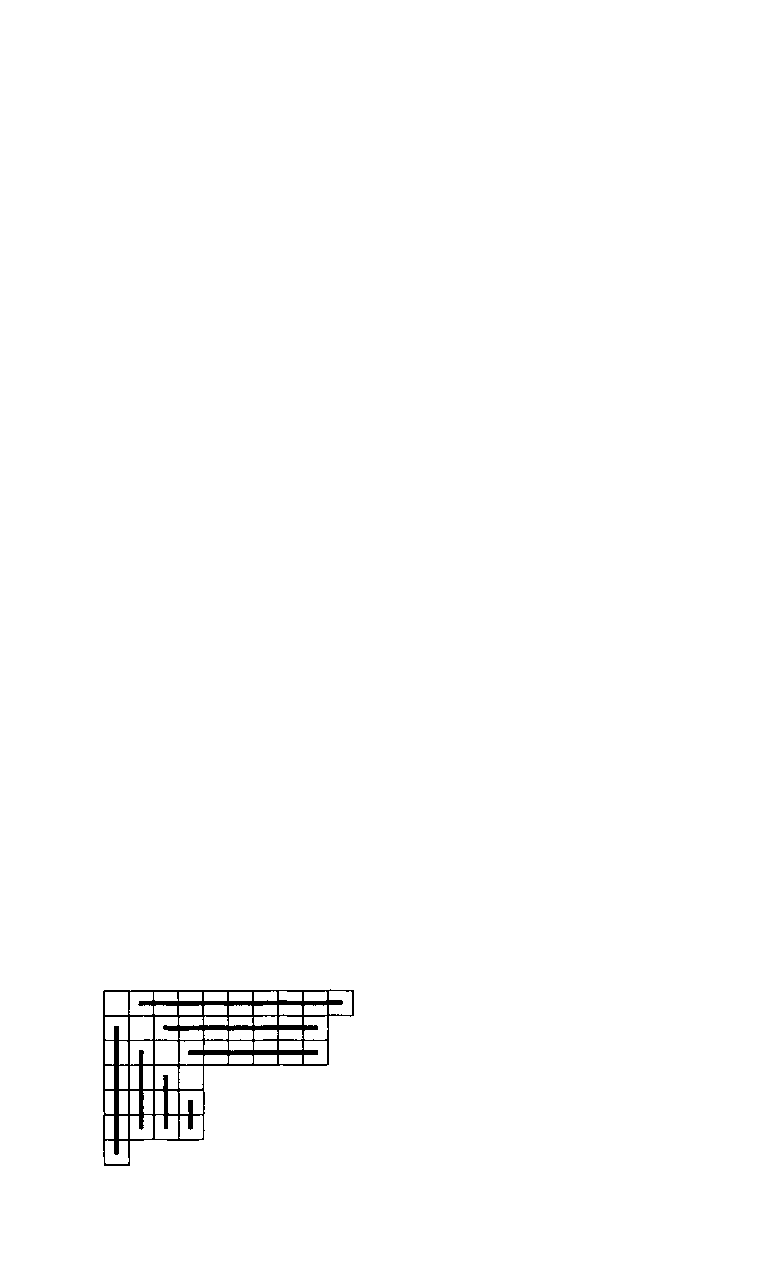
\includegraphics[]{../figures/FH-pag-51.pdf} &\raisebox{1.5cm}{$\begin{matrix*}[l]\l=(10,9,9,4,4,4,1)\\\text{Frobenius notation }\begin{pmatrix}9&7&6&0\\2&3&4&5\end{pmatrix}\\\text{modified Frobenius notation }\begin{pmatrix}9.5&7.5&6.5&0.5\\2.5&3.5&4.5&5.5\end{pmatrix}\end{matrix*}$}\end{matrix}\]

Let also define the \emph{modified Frobenius notation} to be $\begin{pmatrix}a'_1a'_2\ldots a'_n\\b'_1b'_2\ldots b'_n\end{pmatrix}$ where $a'_i=a_i+1/2$ and $b'_i=b_i+1/2$. Then
	
\begin{lemma}[Frobenius formula {\cite[Ex. 4.17(c)]{FH}}]
	\deq{\c^\l(C_{(2)})=\frac{\dim\l}{d(d-1)}\sum_{i=1}^r(a_i(a_i+1)-b_i(b_i+1))=\frac{\dim\l}{d(d-1)}\sum_{i=1}^r((a'_i)^2-(b'_i)^2)}
\end{lemma}

From this and $|C_{(2)}|=\begin{pmatrix}d\\2\end{pmatrix}$ it follows that 
\deq{f_2(\l)=\frac{|C_{(2)}|}{\dim \l}\c^\l(C_{(2)})=\frac12\sum_{i=1}^r((a'_i)^2-(b'_i)^2)}

Draw the Young diagram of $\l$ rotated by $135^\circ$ over the real line with opposite orientation as in the picture and consider the black and white stones as showed. 

\[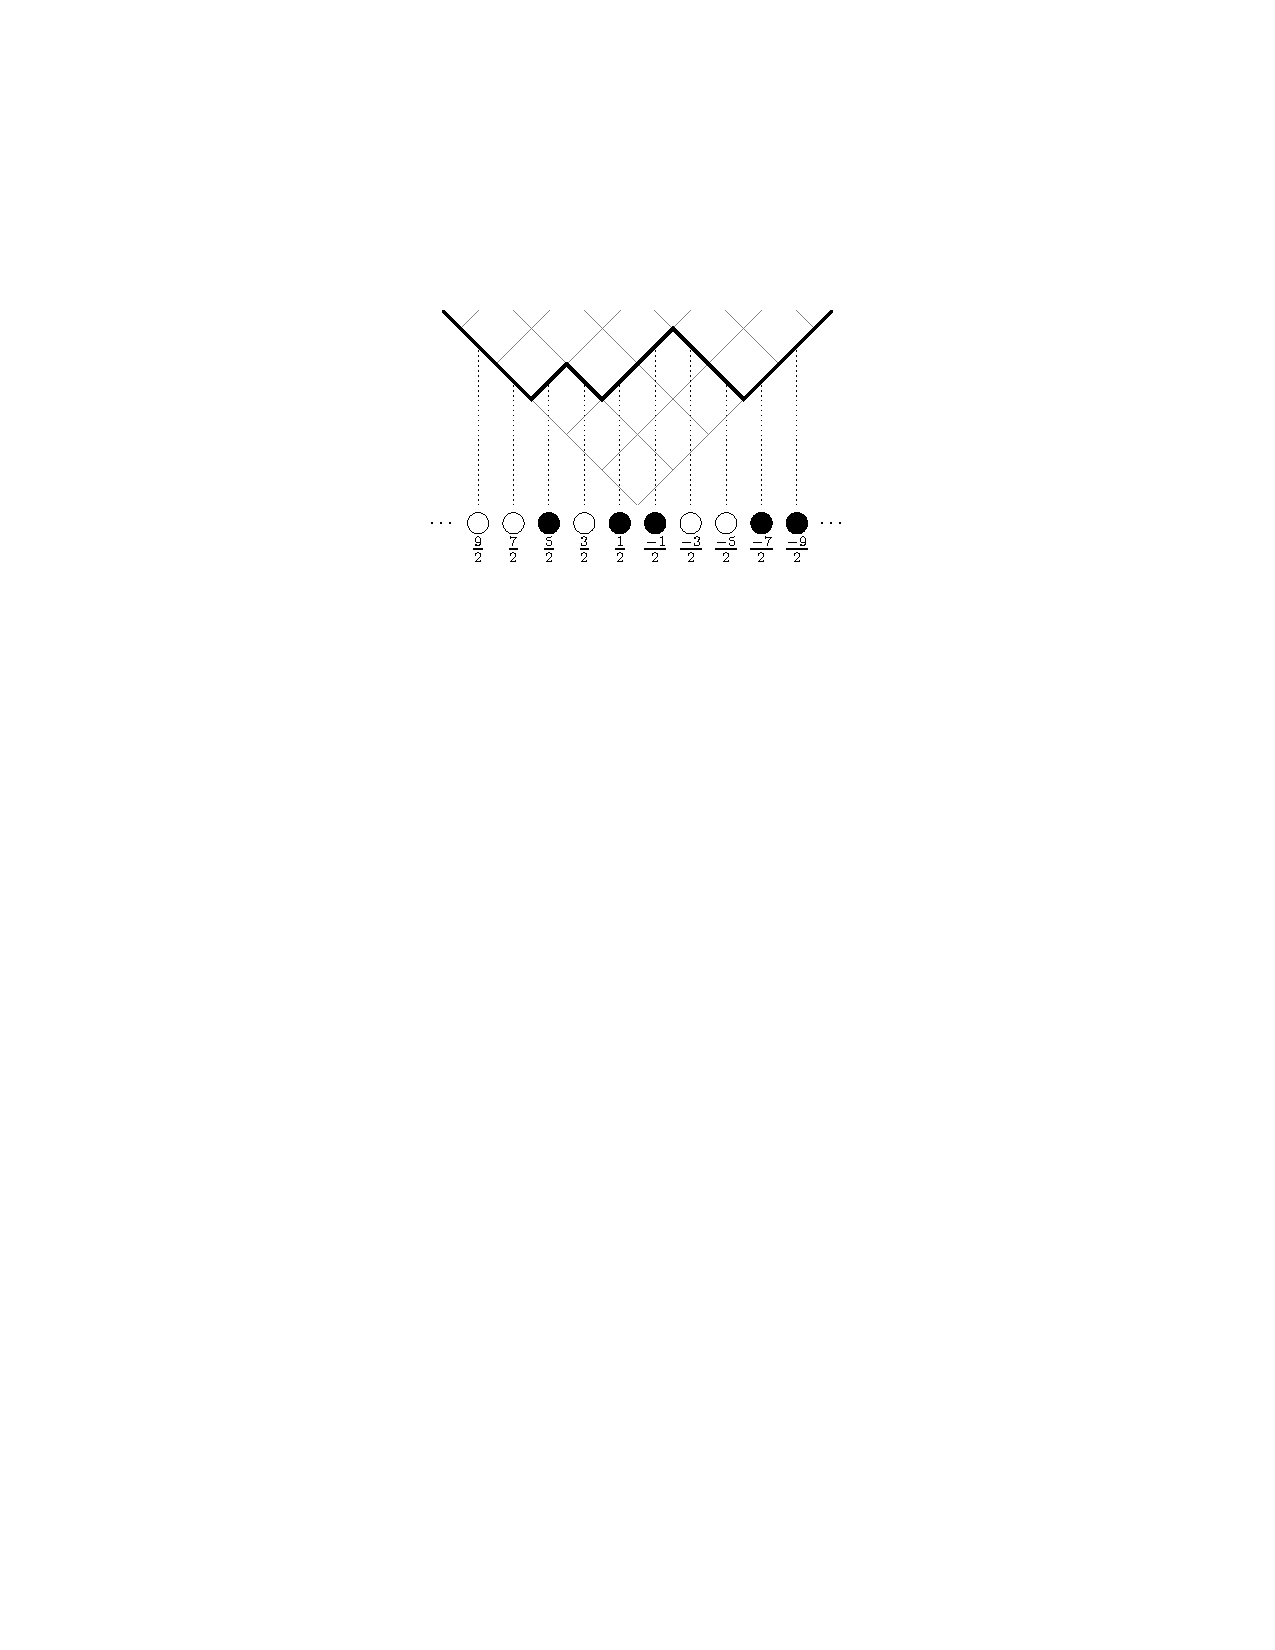
\includegraphics[]{../figures/J-fig-1.pdf}\]

Suppose that $\l$ is made of $k=\ell(\l)$ cycles of lengths $\{\l_1,\ldots,\l_k\}$ where $\l_1\geq\l_2\geq\ldots$. Now consider the ordered set $\{\ti\l_i\}_{i\in\Z_{\geq0}}=\{\l_1,\ldots,\l_k,0,0,\ldots\}$ ending with infinitely many zeros. Then it is clear that black stones are placed in correspondence to elements of 
\deq{\fS_\bullet(\l):=\{\ti\l_i-i+1/2\}\subset\Z+\frac12}
and white stones in correspondence to elements of $\fS_\circ(\l):=(\Z+\frac12)\setminus\fS_\bullet(\l)$. Moreover, the coefficients in the modified Frobenius notation are given by
\deq{\{a'_i\}&=\fS_\bullet^+(\l):=\fS_\bullet\cap(\Z_{\geq0}+1/2)\\
	\{b'_i\}&=\fS_\circ^-(\l):=\fS_\circ\cap(\Z_{\leq0}-1/2)=(\Z_{\leq0}-1/2)\setminus\fS_\bullet(\l)}
Hence we obtained
\deq{f_2(\l)=\sum_{k\in\fS_\bullet^+}\frac{k^2}2-\sum_{k\in\fS_\circ^-}\frac{k^2}2}

Notice also that
\deq{|\l|=\l_1+\cdots+\l_k=a_1'+\cdots+a_k'+b_1'+\cdots+b_k'=\sum_{k\in\fS_\bullet^+} k-\sum_{k\in\fS_\circ^-}k}

The aim of the following section is to write the formula of double Hurwitz numbers and those for the corresponding potentials in terms of matrix elements in the half infinite wedge space. This half infinite wedge space corresponds to the space of possible configurations of black and white stones as before.

\section{Half infinite wedge formalism}

Now we introduce the \emph{half infinite wedge formalism}, also known as \emph{infinite wedge formalism}. As a references see \cite{MJD,O2,J}.

Let $V$ be a vector space with basis $\{\und k\}$, $k\in\Z+\frac12$. We define the vector space $\hiw$ to be spanned by vectors
\deq{v_S:=\und{s_1}\V\und{s_2}\V\und{s_3}\V\ldots}
where $S=\{s_1>s_2>\dots\}\subset\Z+\frac12$ is a subset \st both
\deq{S^+=S\setminus\Big(\Z_{\leq0}-\frac12\Big)\tand S^-=\Big(\Z_{\leq0}-\frac12\Big)\setminus S}
are finite. We equip $\hiw$ with the inner product $(-,-)$ in which the basis $\{v_S\}$ (for all possible choices of $S$) is orthonormal. 

For our purposes $S$ is identified with $\fS_\bullet(\l)$ defined before, we denote by $v_\l$ the vector in $\hiw$ corresponding to $S=\fS_\bullet(\l)$. In this case $S^+=\fS_\bullet^+$ and $S^-=\fS_\circ^-$, and finiteness condition simply corresponds to the fact that we have finitely many black stones on the left of the origin and finitely many white stones on the right or the origin, which is automatic for $\fS_\bullet(\l)$. 

Define the operators $\p_k$ and $\p_k^*$ on $\hiw$ as follows. For $v\in\hiw$ let
\deq{\p_k(v):=\und k\V v}
and let $\p_k^*$ to be the adjoint operator, that is \st
\deq{(v',\p^*_kv)=(\p_kv',v)}
From the definition of these operators and of the inner product, note that they satisfy
\deq{\p_j\p_k^*+\p_k^*\p_j&=\d_{jk}\\
	\p_j\p_k+\p_k\p_j&=0\\
	\p_j^*\p_k^*+\p_k^*\p_j^*&=0}
which are known as \emph{fermionic commutation relations}. 

These operators are related to the usual creation and annihilation operators for the \emph{Fermi sea}, by identifying black stones with electrons and white stones with empty energy levels (but note that in usual physical literature, and in \cite{MJD}, one should exchange $\p_k\leftrightarrow\p_k^*$). Finiteness condition amounts to requiring that the considered state is a finite energy excitation of the vacuum in the Fermi sea. We identify the vacuum of the Fermi sea with the vector $\vac=\und{-\frac12}\V\und{-\frac32}\V\und{-\frac52}\V\ldots$, where all stones are black (resp. white) on the right (resp. left) of the origin.

To see this, note that if $\und k$ is not present in $v_S$ (``the energy level $k$ is empty'') then $\p_k$ add that vector to $v_S$ (''creates the electron'') whereas $\p_k^*$ maps $v_S$ to 0 (``the state is annihilated''). Instead, if $\und k$ is present in $v_S$ (``the energy level $k$ is occupied'') then $\p_k$ maps $v_S$ to 0 (``Pauli principle'') whereas $\p_k^*$ removes that vector from $v_S$ (``the electron at the energy level $k$ is annihilated''). 

Note also that all the vectors in $\hiw$ can be obtained from $\vac$ by applying creation and annihilation operators a finite number of times, that is $\vac$ is cyclic. 

Introduce the \emph{normal ordered product}
\deq{\no{\p_j\p_k^*}\ \ :=\begin{cases}\p_j\p_k^*\quad&k>0\\-\p_k^*\p_j\quad&k<0\end{cases}}
For $k>0$ (resp. $k<0$), $\no{\p_k\p_k^*}$ gives 1 if we have a black (resp. white) stone in $k$ and zero otherwise. For $j\neq k$ the normal ordered product is the ordinary product due to the fermionic commutation relation $\no{\p_j\p_k^*}\ =\p_j\p_k^*=-\p_k^*\p_j$. The effect of $\no{\p_j\p_k^*}\ $ for $j\neq k$ is to take the black stone in $k$ and move it to the position $j$, unless there is no black stone in $k$ or the position $j$ is already occupied: in such cases it gives the zero vector. Finiteness condition ensures that any operator of the form $\sum_{j,k}a_{jk}\no{\p_j\p_k^*}$ is well defined for any choice of the coefficients $a_{j,k}$. Note that the assignement $E_{jk}\mapsto\ \no{\p_j\p_k^*}$ can be understood as a projective representation of $\fgl(V)$ on $\hiw$. 

Now we can define the operator $\cF_2$ 
\deq{\cF_2=\sum_{k\in\Z+\frac12}\frac{k^2}2\no{\p_k\p_k^*}}
which satisfies
\deq{\cF_2v_\l=f_2(\l)v_\l}

Let's see how we can rewrite the whole quantities
\deq{H^\bullet_{d,b}(\q,\q')&=\frac1{\fz(\q)\fz(\q')}\sum_{\l\prt d}\c^\l_{\q}f_2(\l)^b\c^\l_{\q'}\\
	\fh^\bullet_d(\q,\q')&=\frac1{\fz(\q)\fz(\q')}\sum_{\l\prt d}\c^\l_{\q}e^{z f_2(\l)}\c^\l_{\q'}\\
	\fH^\bullet(\{p_j,p_j'\},q,z)&=\sum_{\l}q^{|\l|} s_\l(P)e^{z f_2(\l)}s_\l(P')}
in the half infinte wedge space. To do so we should be able to rewrite also quantities $|\l|$, $\c^\l_\q$ and $s_\l(P)$ in terms of matrix elements in the half infinite wedge space. 

We introduce the following operators, called \emph{energy operator} and \emph{charge operator} respectively
\deq{H:=\sum_{k\in\Z+1/2}k\no{\p_k\p_k^*}
	\qquad
	C:=\sum_{k\in\Z+1/2}\no{\p_k\p_k^*}}
The physical interpretation of these operators is obvious when we regard a black stone at position $k>0$ as an electron of energy $k$ and charge $+1$ and a white stone at position $k<0$ as a positron of energy $-k$ and charge $-1$. 

First notice that from our previous discussion we have 
\deq{Hv_\l=|\l|v_\l}
and so 
\deq{q^He^{z \cF_2}v_\l=q^{|\l|}e^{f_2(\l)}v_\l}


We have 
\deq{Cv_S=(|S^+|-|S^-|)v_s}
Suppose $v_S$ is of charge $c$, \ie $Cv_S=c\,v_S$, then $|S^+|=|S^-|+c$. Pick $k\in S$, $k<\min (S^-)$, this means that the stone at $k$ and all those on its right are black. Then $|S^+|=|S^-|+c$ implies that $k=s_{-(k-1/2)+c}$. Hence the charge of the vector $v_S$ is given by
\deq{c=\lim_{i\to+\infty}\Big(s_i+i-\frac12\Big)}
In particular, all vectors corresponding to Young diagrams ($S=\fS_\bullet(\l)$) have zero charge. Conversely, any vector of zero charge can be obtained from a Young diagram by taking the partition $\l_i=s_i+i-\frac12$ (omitting the infinitely many $\l_i$ which vanish). We denote by $\hiwz$ the subspace of $\hiw$ of zero charge. From this we get that 
\deq{\{v_\l\,\big|\,\l\prt d\}}
is a basis for the subspace of $\hiwz$ given by vectors of energy $d$. Considering all positive values of $d$ we get a basis of the whole charge zero subspace $\hiwz$. 

Now define the following operators for all $n\in\Z_{\neq0}$
\deq{\a_n:=\sum_{k\in\Z+\frac12}\no{\p_{k-n}\p^*_k}}
satisfying $\a_n\und k=\und{k-n}$ and the \emph{Heisenberg commutation relations}\footnote{Note that we realized operators satisfying the \emph{bosonic} algebra using operators satisfying the \emph{fermionic} one. Indeed we have an isomorphism of vector spaces given by $v_\l\leftrightarrow s_\l$ called \emph{Boson-Fermion correspondence}, and the operators $\a_n$ essentially realize some natural bosonic operators in the space of Schur polynomials as operators in the fermionic space $\hiwz$. The correspondence $v_\l\leftrightarrow s_\l$ is the essence of the strong relation between representation theory of $S_d$ and the infinite wedge formalism. See \cite{MJD} for details.}
\deq{[\a_n,\a_m]=n\d_{n+m,0}}
From the definition it follows that $\a_n$ and $\a_{-n}$ are adjoint for every $n\in\Z_{\neq0}$.

The effect of this operator in a certain configuration of stones (or electrons) is the following. Pick one and move it to the right by $n$ positions. If the new position is a white stone, make it black and replace the initial black stone by a white one. If the new position is occupied by a black stone, then the operator gives the zero vector (Pauli principle). Then repeat this for all black stones and sum all the resulting vectors to give the final state. Finiteness condition ensures that this operation is well defined. 

For any partition $\q=\{\q_1,\ldots,\q_{\ell(\q)}\}\prt|\q|$ define
\deq{\a_{\q}:=\prod_{i=1}^{\ell(\q)}\a_{\q_i}
	\tand
	\a_{-\q}:=\prod_{i=1}^{\ell(\q)}\a_{-\q_i}} 
The Heisenberg commutation relation ensures that the ordering of the multiplied operators is not relevant and also that $\a_\q$ and $\a_{-\q}$ are adjoint. Note also that $\a_{\q}$ (resp. $\a_{-\q}$) decreases (resp. increases) the energy of states by $|\q|$. Moreover, it is possible to prove\footnote{\cite[Lemma 2.12]{J}} that 
\deq{\{\a_{-\q}\vac\,\big|\,\q\prt d\}}
is a basis for the subspace of $\hiwz$ of energy $d$, orthogonal \wrt the inner product $(-,-)$. To see this it suffices to prove that $\a_{\q'}\a_{-\q}\vac\propto \d_{\q,\q'}\vac$.

The two bases of $\hiwz$ can be related as follows. Let $\l$ be any partition and $n\in\Z_{>0}$. From the following picture
\[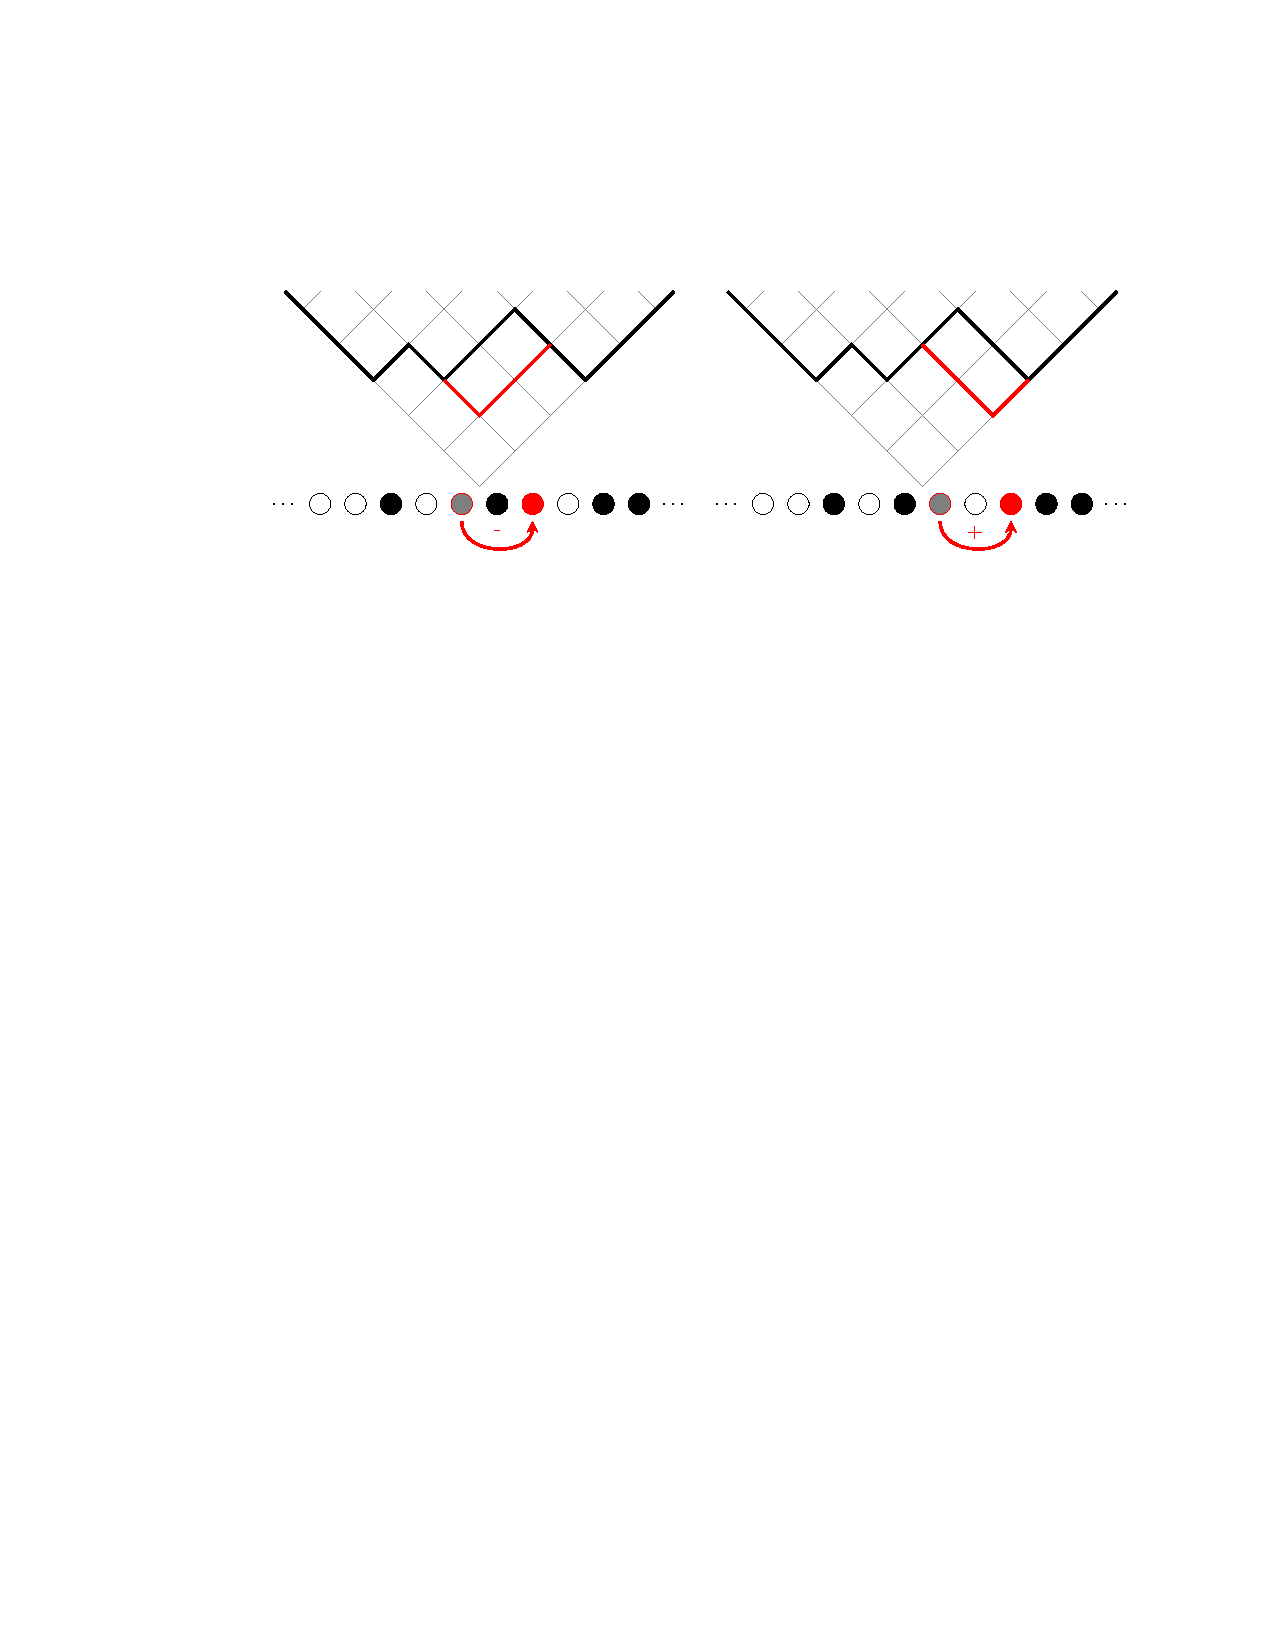
\includegraphics[width=\textwidth]{../figures/J-fig-2.pdf}\]
we can see that 
\deq{\a_{n}v_\l=\sum_{\l'<\l\atop{\text{$\l/\l'$ skew hook}\atop{|\l/\l'|=n}}}(-1)^{r(\l'/\l)-1}v_{\l'}}
where $\l'<\l$ means that $\l'_i<\l_i$ for all $i\leq\ell(\l)$ and $r(\l'/\l)$ is the number of rows of $\l'$ touched by $\l'/\l$. This is very similar to
\begin{lemma}[\emph{Murnaghan-Nakayama rule} {\cite[Ex. 4.45]{FH}}]
	\deq{\c^\l_{\{(n),\q\}}=\sum_{\l'<\l\atop{\text{$\l/\l'$ skew hook}\atop{|\l/\l'|=n}}}(-1)^{r(\l'/\l)-1}\c^{\l'}_\q}
\end{lemma}
Using these identities we get that for any two partitions $\l$ and $\q$ such that $|\l|=|\q|$ 
\deq{\a_{\q} v_\l=\c_\q^\l v_\emptyset}
and than taking the adjoint\footnote{Write $\a_{-\q}\vac=\sum_{\l\prt|\q|}(v_\l,\a_{-\q}\vac)v_\l=\sum_{\l\prt|\q|}(\a_\q v_\l,\vac)v_\l$.} we arrive at
\deq{\a_{-\q}\vac=\sum_{\l\prt |\q|}\c_\q^\l v_\l}

Using this result, for $\q=\{\q_1,\ldots,\q_{\ell(\q)}\}\prt d$ and $\q'=\{\q'_1,\ldots,\q'_{\ell(\q')}\}\prt d$ we obtain
\deq{\big(\vac,\a_\q \cF_2^b\a_{-\q'}\vac\big)
	&=\sum_{\l\prt d}\c_{\q'}^\l\big(\vac,\a_\q \cF_2^b v_\l\big)
	=\sum_{\l\prt d}f_2(\l)^b\c_{\q'}^\l\big(\vac,\a_\q v_\l\big)\\
	&=\sum_{\l\prt d}\c_\q^\l f_2(\l)^b\c_{\q'}^\l\big(\vac,\vac\big)
	=\sum_{\l\prt d}\c_{\q}^{\l}f_2(\l)^b\c_{\q'}^{\l}}
Finally we get
\deq{H^\bullet_{d,b}(\q,\q')&=\frac1{\fz(\q)\fz(\q')}\sum_{\l\prt d}\c^\l_{\q}f_2(\l)^b\c^\l_{\q'}=\frac1{\fz(\q)\fz(\q')}\big\la\a_\q \cF_2^b\a_{-\q'}\big\ra}
where the \emph{correlator} of the operator $A$ is defined by $\la A\ra:=(v_\emptyset,Av_\emptyset)$. Similarly
\deq{\fh^\bullet_d(\q,\q')&=\frac1{\fz(\q)\fz(\q')}\sum_{\l\prt d}\c^\l_{\q}e^{z f_2(\l)}\c^\l_{\q'}=\frac1{\fz(\q)\fz(\q')}\big\la\a_\q e^{z\cF_2}\a_{-\q'}\big\ra}


Now it remains to rewrite
\deq{\fH^\bullet(\{p_j,p_j'\},q,z)&=\sum_{\l}q^{|\l|} s_\l(P)e^{z f_2(\l)}s_\l(P')}
To do so we should be able to recover the Schur polynomials from the half infinite wedge formalism. 

Given a sequence $t=(t_1,t_2,\ldots)$ define
\deq{\G_\pm(t)=\exp\Bigg(\sum_{n=1}^\infty t_n\a_{\pm n}\Bigg)}
Note that $\G_+(t)$ and $\G_-(t)$ are adjoint. The following result can also be related to some results in representation theory of $S_d$
\begin{lemma}[{\cite[Eq. (A.16)]{O2}}, {\cite{MJD}}]
	Consider a set of variables $P=(p_1,p_2,\ldots)$ and denote $p^{(k)}=p_1^k+p_2^k+\cdots$. Then
	\deq{\G_-\bigg(p^{(1)},\frac{p^{(2)}}2,\frac{p^{(3)}}3,\cdots\bigg)\vac=\sum_\l s_\l(P)v_\l}
	where $\sum_\l$ runs over all possible partitions (of any number).
\end{lemma}
Introduce the following abbreviations
\deq{\G_+:=\G_+\bigg(p^{(1)},\frac{p^{(2)}}2,\frac{p^{(3)}}3,\cdots\bigg)
	\tand
	\G_-:=\G_-\bigg(p'^{(1)},\frac{p'^{(2)}}2,\frac{p'^{(3)}}3,\cdots\bigg)}
where $P=(p_1,p_2,\ldots)$, $P'=(p'_1,p'_2,\ldots)$. 
Using the lemma we have
\deq{&\big(\vac,\G_+q^He^{z \cF_2}\G_-\vac\big)
	=\big(\G_-\vac,q^He^{z \cF_2}\G_-\vac\big)
	=\sum_{\l,\l'}s_\l(P)s_{\l'}(P')\big(v_\l,q^He^{z \cF_2}v_{\l'}\big)\\
	&\qquad=\sum_{\l,\l'}s_\l(P)e^{z f_2(\l')}s_{\l'}(P')\big(v_\l,q^Hv_{\l'}\big)
	=\sum_{\l,\l'}q^{|\l'|}s_\l(P)e^{z f_2(\l')}s_{\l'}(P')\big(v_\l,v_{\l'}\big)\\
	&\qquad=\sum_{\l}q^{|\l|}s_\l(P)e^{z f_2(\l)}s_{\l}(P')}
so
\deq{\fH^\bullet(\{p_j,p_j'\},q,z)=\big\la\G_+q^He^{z \cF_2}\G_-\big\ra}

Summarizing, we obtained the following formulas
\deq{H^\bullet_{d,b}(\q,\q')&=\frac1{\fz(\q)\fz(\q')}\big\la\a_\q \cF_2^b\a_{-\q'}\big\ra\\
	\fh^\bullet_d(\q,\q')&=\frac1{\fz(\q)\fz(\q')}\big\la\a_\q e^{z\cF_2}\a_{-\q'}\big\ra\\
	\fH^\bullet(\{p_j,p_j'\},q,z)&=\big\la\G_+q^He^{z \cF_2}\G_-\big\ra}
The last one was first derived in \cite{O1}, and later the first two were derived in \cite{OP1} (although in a quite different form). In \cite{O1} it was shown also that the Hurwitz potential $\fH^\bullet$ is the $\w$-function for the Toda lattice hierarchy of Ueno and Takasaki, implying (infinitely) many recursive relations on $\fH^\bullet$. The technique applied here was later generalized to Gromov-Witten theory in \cite{OP1,OP2}. 

Notice that, by considering the energies of the operators in the correlators, it is clear that we should have $|\q|=|\q'|$ in order to have nonzero values, as expected since we should have $|\q|=d=|\q'|$. 

Introducing other operators it is possible to rewrite the previous correlators in such a way that their explicit computation is much simplified. See \cite{J,OP1,OP2} for more details. In order to simplify the notation, denote
\deq{E_{ij}=\ \no{\p_j\p_k^*}}

\begin{definition}
	Let $r\in\Z$. We define
	\deq{\cE_r(z):=\sum_{k\in\Z+\frac12}e^{z(k-r/2)}E_{k-r,k}+\frac{\d_{r,0}}{\varsigma(z)}}
	where
	\deq{\varsigma(z):=e^{z/2}-e^{-z/2}}
\end{definition}

Let's explain the meaning of the additional term arising when $r=0$. We would like to have an operator which acts as
\deq{\und k\mapsto e^{zk}\und{k}}
and the natural candidate is 
\deq{\sum_{k\in\Z+\frac12}e^{zk}\p_{k}\p_k^*}
However applying it to the vacuum the second definition gives for $\Re z>0$
\deq{\sum_{k\in\Z_{\leq0}-\frac12}e^{zk}=e^{-z/2}\sum_{k\in\Z_{\leq0}}e^{zk}=\frac{e^{-z/2}}{1-e^{-z}}=\frac1{\varsigma(z)}}
and diverges for $\Re z=0$. So we regularize
\deq{\sum_{k\in\Z+\frac12}e^{zk}\p_{k}\p_k^*=\sum_{k\in\Z+\frac12}e^{zk}E_{k,k}+\sum_{k\in\Z_{\leq0}-\frac12}e^{zk} \quad\mapsto\quad \sum_{k\in\Z+\frac12}e^{zk}E_{k,k}+\frac1{\varsigma(z)}}
For $r\neq0$ we don't have any problem since $E_{k-r,k}=\p_{k-r}\p_k^*$.

The exponent $r/2$ in the definition is used in order to have
\deq{\cE_r(z)^*=\cE_{-r}(z)}
The operators $\cE$ satisfy the following commutation relation
\deq{[\cE_a(z),\cE_b(w)]=\varsigma(\det\left[\begin{smallmatrix}a&z\\b&w\end{smallmatrix}\right])\cE_{a+b}(z+w)}
The operators $\cE$ specialize to the standard bosonic operators on $\hiw$
\deq{\a_k=\cE_k(0)\tcomma k\neq0}

\begin{definition}
	For $k\in\Z_{>0}$ define operators $\cF_k$ and $\cP_k$ by
	\deq{\cF_k=\frac{\cP_k}{k!}=[z^k]\cE_0(z)}
	where $[z^k]\cE_0(z)$ stands for the coefficient of $z^k$ in $\cE_0(z)$. 
\end{definition}

\begin{lemma}[{\cite[Eq. 2.11]{OP1}}]
	For $\l=(\l_1,\ldots,\l_k,0,0,\ldots)$ partition
	\deq{\cP_k v_\l={\bf p}_k(\l)v_\l}
	where
	\deq{{\bf p}_k(\l)=\sum_{i=1}^\infty\bigg[\Big(\l_i-i+\frac12\Big)^k-\Big(-i+\frac12\Big)^k\bigg]+(1-2^{-k})\z(-k)}
	where $\z$ is the Riemann zeta function.
\end{lemma}
The meaning of the term $(1-2^{-k})\z(-k)$ is as before, that is we would like to have
\deq{\sum_{i=1}^\infty\Big(\l_i-i+\frac12\Big)^k}
but if we consider the partition $\emptyset$ we get the following divergent contribution
\deq{\sum_{i=1}^\infty\Big(-i+\frac12\Big)^k}
which can be regularized as before giving $(1-2^{-k})\z(-k)$.

Notice that the lemma imply that $\cF_2$ really coincides with the operator defined previously. Indeed we can rewrite the formula above as
\deq{{\bf p}_k(\l)=\sum_{i\in\fS_\bullet^+}{i^k}-\sum_{i\in\fS_\circ^-}{i^k}+(1-2^{-k})\z(-k)}
and $\z(-2)=0$. 

The last formula we need is 
\begin{lemma}[{\cite[Eq. 2.14]{OP2}}]
	\deq{e^{z\cF_2}\a_{-n}e^{-z\cF_2}=\cE_{-n}(nz)}
\end{lemma}

Now we can rewrite the modified Hurwitz potential in a better form which makes computations simpler. Using $\cF_2\vac=0$ we have
\deq{\fh^\bullet_d(\q,\q')&=\frac1{\fz(\q)\fz(\q')}\big\la\a_\q e^{z\cF_2}\a_{-\q'}\big\ra
	=\frac1{\fz(\q)\fz(\q')}\big\la\prod_{i=1}^{\ell(\q)}\a_{\q_i}\prod_{j=1}^{\ell(\q')}\big(e^{z\cF_2}\a_{-\q'_j}e^{-z\cF_2}\big)\ra\\
	&=\frac1{\fz(\q)\fz(\q')}\big\la\prod_{i=1}^{\ell(\q)}\cE_{\q_i}(0)\prod_{j=1}^{\ell(\q')}\cE_{-\q'_j}(z\q'_j)\big\ra}
Using the commutation relation for the operators $\cE$ it is possible to compute the correlator in the previous formula by moving the operators with negative energy on the right and those of positive energy on the left. Then only operators of zero energy survive, so we get a sum of terms of the form $\vars(m_1z)\vars(m_2z)\cdots\cE_0(n_1z)\cE_0(n_2z)\cdots$ for some positive integers $m_1,m_2,\ldots,n_1,n_2,\ldots$.
Now recall
\deq{
	\cE_0(nz)=\sum_{k\in\Z+\frac12}e^{nzk}E_{k-r,k}+\frac1{\vars(nz)}}  
and $E_{k-r,k}\vac=0$ for all $k,r$. Hence $\la\cE_0(nz)\ra=\inv\vars(nz)$ and we get as final result a sum of terms of the form $\vars(m_1z)\vars(m_2z)\cdots\inv\vars(n_1z)\inv\vars(n_2 z)\cdots$.  


\begin{example}
	We illustrate the previous procedure by computing $\fh^\bullet_d(\q,\q')$ when $\q=(\q_1,\q_2)$ and $\q'=(\q'_1,\q'_2)$, satisfying $\q_1+\q_2=\q'_1+\q'_2=d$. We assume $\q_1>\q'_1>\q'_2>\q_2$. Then
	\deq{\fh^\bullet_d(\q,\q')=\frac1{\fz(\q)\fz(\q')}\big\la\cE_{\q_1}(0)\cE_{\q_2}(0)\cE_{-\q'_1}(z\q'_1)\cE_{-\q'_2}(z\q'_2)\big\ra}
	Moving $\cE_{\q_2}(0)$ to the right we have
	\deq{&\big\la\cE_{\q_1}(0)\cE_{\q_2}(0)\cE_{-\q'_1}(z\q'_1)\cE_{-\q'_2}(z\q'_2)\big\ra=\\
		&\quad=\big\la\cE_{\q_1}(0)\cE_{-\q'_1}(z\q'_1)\cE_{\q_2}(0)\cE_{-\q'_2}(z\q'_2)\big\ra+\vars(z\q_2\q'_1)\big\la\cE_{\q_1}(0)\cE_{\q_2-\q'_1}(z\q'_1)\cE_{-\q'_2}(z\q'_2)\big\ra}
	Moving again $\cE_{\q_2}(0)$ to the right in the first term we get
	\deq{&\big\la\cE_{\q_1}(0)\cE_{-\q'_1}(z\q'_1)\cE_{\q_2}(0)\cE_{-\q'_2}(z\q'_2)\big\ra=\\
		&\quad=\big\la\cE_{\q_1}(0)\cE_{-\q'_1}(z\q'_1)\cE_{-\q'_2}(z\q'_2)\cE_{\q_2}(0)\big\ra+\vars(z\q_2\q_2')\big\la\cE_{\q_1}(0)\cE_{-\q'_1}(z\q'_1)\cE_{\q_2-\q'_2}(z\q'_2)\big\ra}
	The first term vanish since $\cE_{\q_2}(0)$ has negative energy. Similarly
	\deq{&\big\la\cE_{\q_1}(0)\cE_{\q_2-\q'_1}(z\q'_1)\cE_{-\q'_2}(z\q'_2)\big\ra=\\
		&\quad=\big\la\cE_{\q_2-\q'_1}(z\q'_1)\cE_{\q_1}(0)\cE_{-\q'_2}(z\q'_2)\big\ra+\vars(z\q_1\q'_1)\big\la\cE_{\q_1+\q_2-\q'_1}(z\q'_1)\cE_{-\q'_2}(z\q'_2)\big\ra}
	and
	\deq{&\big\la\cE_{\q_1}(0)\cE_{-\q'_1}(z\q'_1)\cE_{\q_2-\q'_2}(z\q'_2)\big\ra=\\
		&\quad=\big\la\cE_{-\q'_1}(z\q'_1)\cE_{\q_1}(0)\cE_{\q_2-\q'_2}(z\q'_2)\big\ra+\vars(z\q_1\q'_1)\big\la\cE_{\q_1-\q'_1}(z\q'_1)\cE_{\q_2-\q'_2}(z\q'_2)\big\ra}
	where the first terms vanish since $\cE_{\q_2-\q'_1}(z\q'_1)$ and $\cE_{-\q'_1}(z\q'_1)$ have positive energy. It remains to consider
	\deq{&\big\la\cE_{\q_1+\q_2-\q'_1}(z\q'_1)\cE_{-\q'_2}(z\q'_2)\big\ra=\\
		&\quad=\big\la\cE_{-\q'_2}(z\q'_2)\cE_{\q_1+\q_2-\q'_1}(z\q'_1)\big\ra+\vars\big[z((\q_1+\q_2-\q'_1)\q'_2-(-\q'_2)\q'_1)\big]\big\la\cE_{\q_1+\q_2-\q'_1-\q'_2}(z(\q'_1+\q'_2))\big\ra=\\
		&\quad=\vars(zd\q'_2)\big\la\cE_0(zd)\big\ra}
	and
	\deq{&\big\la\cE_{\q_1-\q'_1}(z\q'_1)\cE_{\q_2-\q'_2}(z\q'_2)\big\ra=\\
		&\quad=\big\la\cE_{\q_2-\q'_2}(z\q'_2)\cE_{\q_1-\q'_1}(z\q'_1)\big\ra+\vars\big[z((\q_1-\q'_1)\q'_2-(\q_2-\q'_2)\q'_1)\big]\big\la\cE_{\q_1-\q'_1+\q_2-\q'_2}(z(\q'_1+\q'_2))\big\ra\\
		&\quad=\vars(z(\q_1\q'_2-\q_2\q'_1))\big\la\cE_0(zd)\big\ra}
	Putting our results together
	\deq{&\big\la\cE_{\q_1}(0)\cE_{\q_2}(0)\cE_{-\q'_1}(z\q'_1)\cE_{-\q'_2}(z\q'_2)\big\ra=\\
		&\quad=\vars(z\q_2\q_2')\vars(z\q_1\q'_1)\vars(z(\q_1\q'_2-\q_2\q'_1))\big\la\cE_0(zd)\big\ra+\vars(z\q_2\q'_1)\vars(z\q_1\q'_1)\vars(zd\q'_2)\big\la\cE_0(zd)\big\ra\\
	&\quad=\frac{\vars(z\q_2\q_2')\vars(z\q_1\q'_1)\vars(z(\q_1\q'_2-\q_2\q'_1))+\vars(z\q_2\q'_1)\vars(z\q_1\q'_1)\vars(zd\q'_2)}{\vars(zd)}}
	and using the following identity for $\vars$ 
	\deq{\vars(a-b)\vars(c)+\vars(b-c)\vars(a)+\vars(c-a)\vars(b)=0}
	we finally get
	\deq{\fh^\bullet_d(\q,\q')=\frac1{\fz(\q)\fz(\q')}\frac{\vars(z\q_1\q'_1)\vars(z\q_1\q'_2)\vars(z\q_2d)}{\vars(zd)}}
\end{example}


\end{document}